% ============================================================
%  CALASH -- 20-minute PhD Presentation
%  Beamer + Metropolis theme (clean, modern)
% ============================================================
\documentclass[aspectratio=169, 11pt]{beamer}

% --- Theme ---
\usetheme{Madrid}
\usecolortheme{default}
\setbeamertemplate{navigation symbols}{}
\setbeamertemplate{footline}{%
  \leavevmode\hbox{%
    \begin{beamercolorbox}[wd=.33\paperwidth,ht=2.5ex,dp=1ex,center]{author in head/foot}%
      \usebeamerfont{author in head/foot}\insertshortauthor
    \end{beamercolorbox}%
    \begin{beamercolorbox}[wd=.34\paperwidth,ht=2.5ex,dp=1ex,center]{title in head/foot}%
      \usebeamerfont{title in head/foot}\insertshorttitle
    \end{beamercolorbox}%
    \begin{beamercolorbox}[wd=.33\paperwidth,ht=2.5ex,dp=1ex,right]{date in head/foot}%
      \usebeamerfont{date in head/foot}\insertdate\hspace*{2em}
      \insertframenumber{}/\inserttotalframenumber\hspace*{2ex}
    \end{beamercolorbox}}%
  \vskip0pt%
}

% --- Packages ---
\usepackage[T1]{fontenc}
\usepackage[utf8]{inputenc}
\usepackage{amsmath,amsfonts}
\usepackage{booktabs}
\usepackage{graphicx}
\usepackage{multirow}
\usepackage{pifont}    % \ding{51} checkmark, \ding{55} cross
\usepackage{tikz}
\usetikzlibrary{positioning, arrows.meta, decorations.pathreplacing, calc}
\usepackage{adjustbox}
\usepackage{array}
\usepackage{colortbl}
\usepackage{xcolor}
\usepackage{enumitem}          % nosep, topsep control in lists
\setitemize{label=\usebeamertemplate{itemize item}}

\graphicspath{{CALASH/figures/}}

% --- Custom colours ---
\definecolor{calash}{RGB}{0,100,170}
\definecolor{alertred}{RGB}{200,40,40}
\definecolor{okgreen}{RGB}{40,140,40}
\definecolor{lightgray}{gray}{0.92}
\definecolor{tablegray}{gray}{0.95}

% shorthand
\newcommand{\cmark}{\textcolor{okgreen}{\ding{51}}}
\newcommand{\xmark}{\textcolor{alertred}{--}}
\newcommand{\CO}{CO\textsubscript{2}}
\newcommand{\LCI}{\text{LCI}}

% --- Meta ---
\title[CALASH]{Carbon-Aware Lifecycle-Adaptive Self-Healing Routing\\for 6G-Integrated Disaster Sensor Networks}
\subtitle{2nd Article -- PhD Research Presentation}
\author[G.~Djimefo]{Georges Djimefo \and Raaa Mamam \and Sasam Pasda \and Frama Aldo}
\institute{Polytechnique Montr\'{e}al -- LARIM}
\date{March 11, 2026}
\titlegraphic{
\includegraphics[height=1cm]{Larim_logo.png}\hspace{1.5cm}
\includegraphics[height=1cm]{Polytechnique_Montreal_Logo.jpg}}

\begin{document}

% ============================================================
%  TITLE
% ============================================================
\begin{frame}[plain]
\titlepage
\end{frame}

% ============================================================
%  OUTLINE
% ============================================================
\begin{frame}{Outline}
\tableofcontents
\end{frame}

% %%%%%%%%%%%%%%%%%%%%%%%%%%%%%%%%%%%%%%%%%%%%%%%%%%%%%%%%%%%%
\section{Introduction}
% %%%%%%%%%%%%%%%%%%%%%%%%%%%%%%%%%%%%%%%%%%%%%%%%%%%%%%%%%%%%

\begin{frame}{Introduction -- Context: WSNs and Carbon Footprint}
\begin{columns}[T]
\column{0.55\textwidth}
\begin{itemize}
    \item \textbf{WSNs}: hundreds of battery-powered sensors ($E_0 = 0.5$\,J)
    \item ICT sector: \textbf{2--4\% of global GHG emissions} (comparable to aviation)
    \item IoT is the fastest-growing ICT segment
    \item \textbf{Embodied carbon dominates}: $\sim$10\,kg\,\CO eq/node vs.\ $\sim$0.01\,g operational
    \item Disaster events can destroy 30--50\% of nodes instantly
\end{itemize}
\column{0.42\textwidth}
\centering
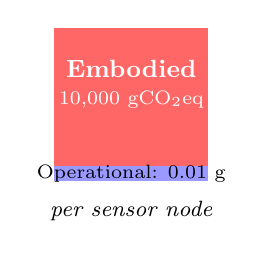
\begin{tikzpicture}[scale=0.65, every node/.style={font=\scriptsize}]
    % Pie-like visual for carbon
    \fill[red!60] (0,0) rectangle (3,3);
    \node[white, font=\small\bfseries] at (1.5,2.2) {Embodied};
    \node[white] at (1.5,1.6) {10,000 g\CO eq};
    \fill[blue!40] (0,0) rectangle (3,0.3);
    \node at (1.5,0.15) {Operational: 0.01 g};
    \node[below, font=\footnotesize\itshape] at (1.5,-0.2) {per sensor node};
\end{tikzpicture}

\vspace{3mm}
\textbf{Key insight:} Maximize delivered packets\\= minimize carbon per packet
\end{columns}
\end{frame}

\begin{frame}{Introduction -- Lifecycle Carbon Intensity (LCI)}
\begin{block}{Novel Metric}
\[
\text{LCI} = \frac{C_{\text{embodied}} + C_{\text{operational}} + C_{\text{end-of-life}}}{\text{total useful packets delivered}} \quad [\text{g\CO eq/pkt}]
\]
\end{block}

\vspace{3mm}
\begin{itemize}
    \item \textbf{Embodied}: manufacturing, assembly, transport ($\sim$10 kg\,\CO eq/node)
    \item \textbf{Operational}: grid carbon intensity $\times$ energy consumed
    \item \textbf{End-of-life}: e-waste disposal ($500 \times (1 - r_{\text{recycle}})$ g\CO eq)
    \item Follows \textbf{ISO 14040 / 14044} lifecycle assessment standards
\end{itemize}

\vspace{3mm}
\centering
\textcolor{calash}{\textbf{Best strategy: send MORE useful packets $\Rightarrow$ lower LCI}}
\end{frame}

% %%%%%%%%%%%%%%%%%%%%%%%%%%%%%%%%%%%%%%%%%%%%%%%%%%%%%%%%%%%%
\section{Related Works}
% %%%%%%%%%%%%%%%%%%%%%%%%%%%%%%%%%%%%%%%%%%%%%%%%%%%%%%%%%%%%

\begin{frame}{Related Works -- Energy-Efficient Clustering \& Metaheuristics}
\centering
\begin{adjustbox}{max width=\textwidth}
\footnotesize
\rowcolors{2}{tablegray}{white}
\begin{tabular}{p{2.4cm} p{3.0cm} p{3.0cm} p{3.0cm} p{3.5cm}}
\toprule
\textbf{Reference} & \textbf{Objective} & \textbf{Methodology} & \textbf{Key Results} & \textbf{Limitations} \\
\midrule
Heinzelman (2000)\newline LEACH & Balanced energy via\newline rotating CHs & Probabilistic CH\newline election threshold & Universal WSN\newline baseline (30k+ cit.) & No carbon, no CS,\newline no disaster recovery \\
Bakaraniya (2013)\newline EE-LEACH & Improve CH selection\newline with residual energy & Energy-weighted\newline threshold & Longer lifetime\newline than LEACH & No multi-hop,\newline no carbon, no CS \\
Younis (2004)\newline HEED & Distributed iterative\newline CH election & Residual energy +\newline communication cost & Better load balance & No carbon,\newline no disaster recovery \\
El Khediri (2024)\newline ABC-ACO & Joint CH selection\newline \& routing & ABC + ACO\newline hybrid metaheuristic & State-of-art\newline meta-heuristic & No carbon awareness,\newline no CS, no self-healing \\
Biswas (2018)\newline EERP & Energy-efficient\newline relay selection & Residual energy +\newline distance to BS & Good energy\newline balance & No carbon, no RL,\newline no disaster recovery \\
\bottomrule
\end{tabular}
\end{adjustbox}
\end{frame}

\begin{frame}{Related Works -- RL-Based Routing \& Recent Advances}
\centering
\begin{adjustbox}{max width=\textwidth}
\footnotesize
\rowcolors{2}{tablegray}{white}
\begin{tabular}{p{2.4cm} p{3.0cm} p{3.0cm} p{3.0cm} p{3.5cm}}
\toprule
\textbf{Reference} & \textbf{Objective} & \textbf{Methodology} & \textbf{Key Results} & \textbf{Limitations} \\
\midrule
Boyan \& Littman\newline (1994) Q-Routing & Online next-hop\newline learning & Tabular Q-learning\newline for routing & Foundational RL\newline routing paper & No carbon, no DNN,\newline no disaster recovery \\
Akram (2025)\newline EEMLCR & ML clustering +\newline energy routing & Machine-learning\newline unified framework & Recent combined\newline approach & No carbon awareness,\newline no LCA integration \\
Wang (2025)\newline Fuzzy-DRL & Distributed cluster\newline routing & Fuzzy logic + deep\newline RL & Decentralized\newline adaptation & No carbon budget,\newline no convergence guarantee \\
Kaur (2025) & Compare clustering\newline protocols & Systematic review\newline of LEACH variants & Confirms energy is\newline sole target & No carbon, no lifecycle\newline perspective \\
\bottomrule
\end{tabular}
\end{adjustbox}
\end{frame}

\begin{frame}{Related Works -- Carbon-Aware Networking \& Disaster/LCA}
\centering
\begin{adjustbox}{max width=\textwidth}
\footnotesize
\rowcolors{2}{tablegray}{white}
\begin{tabular}{p{2.6cm} p{3.0cm} p{3.0cm} p{3.0cm} p{3.3cm}}
\toprule
\textbf{Reference} & \textbf{Objective} & \textbf{Methodology} & \textbf{Key Results} & \textbf{Limitations} \\
\midrule
Freitag (2021) & Quantify ICT carbon\newline footprint & Literature review\newline \& analysis & ICT = 2--4\%\newline global GHG & Cloud/DC scope only,\newline not applied to WSN \\
Huynh (2025) & Carbon-aware edge\newline computing & Digital-twin\newline framework & Reduced carbon in\newline edge workloads & Not for resource-\newline constrained WSNs \\
Erdelj (2017) & Disaster WSN\newline management survey & Survey of protocols & Most assume\newline static topology & No carbon awareness,\newline no LCA \\
Pirson \& Bol (2021) & IoT embodied carbon\newline quantification & Full LCA of IoT\newline devices & Embodied $\gg$ oper.\newline by 3--5 orders & Not integrated into\newline routing decisions \\
Karaman (2025) & 6G-era disaster\newline networks survey & Literature survey & Need for resilient\newline 6G routing & No protocol proposed \\
\bottomrule
\end{tabular}
\end{adjustbox}
\end{frame}

% %%%%%%%%%%%%%%%%%%%%%%%%%%%%%%%%%%%%%%%%%%%%%%%%%%%%%%%%%%%%
\section{Problem Statement}
% %%%%%%%%%%%%%%%%%%%%%%%%%%%%%%%%%%%%%%%%%%%%%%%%%%%%%%%%%%%%

\begin{frame}{Problem Statement -- Four Gaps in the Literature}
\begin{block}{No existing protocol simultaneously addresses all four gaps:}
\end{block}
\vspace{1mm}
\begin{enumerate}[nosep]
    \item[\textcolor{alertred}{\textbf{P1}}] \textbf{No carbon-aware data reduction for WSNs}\\
    {\scriptsize All clustering protocols optimize energy only, ignoring grid carbon intensity ---
    \textit{[Heinzelman 2000, Bakaraniya 2013, Younis 2004, El Khediri 2024, Kaur 2025]}}

    \vspace{1mm}
    \item[\textcolor{alertred}{\textbf{P2}}] \textbf{No provable carbon-budget routing with online learning}\\
    {\scriptsize RL-based routing lacks convergence guarantees on carbon budgets ---
    \textit{[Boyan 1994, Akram 2025, Wang 2025]}}

    \vspace{1mm}
    \item[\textcolor{alertred}{\textbf{P3}}] \textbf{No autonomic disaster self-healing with carbon awareness}\\
    {\scriptsize Disaster protocols assume static topologies; no carbon-aware recovery ---
    \textit{[Erdelj 2017, Alsayyed 2025, Karaman 2025]}}

    \vspace{1mm}
    \item[\textcolor{alertred}{\textbf{P4}}] \textbf{No lifecycle carbon integration in routing objectives}\\
    {\scriptsize Embodied carbon ($\gg$ operational) is never considered in WSN routing ---
    \textit{[Pirson \& Bol 2021, Freitag 2021, Huynh 2025]}}
\end{enumerate}
\end{frame}

\begin{frame}{Problem Statement -- Gap Summary Table}
\centering
\begin{adjustbox}{max width=0.95\textwidth}
\begin{tabular}{lccccccc}
\toprule
\textbf{Feature} & \rotatebox{60}{LEACH} & \rotatebox{60}{EE-LEACH} & \rotatebox{60}{ABC-ACO} & \rotatebox{60}{EERP} & \rotatebox{60}{Q-Routing} & \rotatebox{60}{RIS-DRL} & \rotatebox{60}{\textbf{CALASH}} \\
\midrule
Energy-aware CH       & \cmark & \cmark & \cmark & \cmark & \cmark & \cmark & \cmark \\
Multi-hop routing     & \xmark & \xmark & \cmark & \cmark & \cmark & \cmark & \cmark \\
RL / DQN routing      & \xmark & \xmark & \xmark & \xmark & \cmark & \cmark & \cmark \\
Carbon-aware routing  & \xmark & \xmark & \xmark & \xmark & \xmark & \xmark & \cmark \\
Adaptive compression  & \xmark & \xmark & \xmark & \xmark & \xmark & \xmark & \cmark \\
Disaster self-healing & \xmark & \xmark & \xmark & \xmark & \xmark & \xmark & \cmark \\
Lifecycle LCA         & \xmark & \xmark & \xmark & \xmark & \xmark & \xmark & \cmark \\
Provable guarantees   & \xmark & \xmark & \xmark & \xmark & \xmark & \xmark & \cmark \\
\bottomrule
\end{tabular}
\end{adjustbox}

\vspace{4mm}
\textcolor{calash}{\textbf{CALASH is the only protocol addressing all eight features.}}
\end{frame}

% %%%%%%%%%%%%%%%%%%%%%%%%%%%%%%%%%%%%%%%%%%%%%%%%%%%%%%%%%%%%
\section{Research Questions}
% %%%%%%%%%%%%%%%%%%%%%%%%%%%%%%%%%%%%%%%%%%%%%%%%%%%%%%%%%%%%

\begin{frame}{Research Questions}
\begin{block}{\textbf{Main Question (MQ)}}
\textit{How can a WSN routing protocol jointly minimize lifecycle carbon intensity while maintaining high data delivery and disaster resilience in 6G-integrated sensor networks?}
\end{block}

\vspace{2mm}
\begin{alertblock}{\textbf{Specific Questions}}
\begin{enumerate}[nosep]
    \item[\textbf{SQ1}] How can real-time grid carbon intensity be used to dynamically modulate data compression and routing in resource-constrained WSNs?

    \vspace{1mm}
    \item[\textbf{SQ2}] Can a hybrid Lyapunov--DQN routing framework provide provable carbon-budget guarantees while learning online from experience?

    \vspace{1mm}
    \item[\textbf{SQ3}] How does an autonomic self-healing mechanism (MAPE-K) affect network lifetime and carbon footprint after disaster events?
\end{enumerate}
\end{alertblock}
\end{frame}

% %%%%%%%%%%%%%%%%%%%%%%%%%%%%%%%%%%%%%%%%%%%%%%%%%%%%%%%%%%%%
\section{Objectives}
% %%%%%%%%%%%%%%%%%%%%%%%%%%%%%%%%%%%%%%%%%%%%%%%%%%%%%%%%%%%%

\begin{frame}{Research Objectives}
\begin{block}{\textbf{Main Objective (MO)}}
Design, implement, and evaluate \textbf{CALASH} -- a Carbon-Aware Lifecycle-Adaptive Self-Healing routing framework that minimizes lifecycle carbon intensity for 6G-integrated disaster WSNs.
\end{block}

\vspace{2mm}
\begin{exampleblock}{\textbf{Specific Objectives}}
\begin{enumerate}[nosep]
    \item[\textbf{SO1}] Develop \textbf{CADR} (Carbon-Aware Data Reduction): dynamically tune compressive-sensing ratios inversely to grid carbon intensity.
    \hfill \textit{$\rightarrow$ SQ1}

    \vspace{1mm}
    \item[\textbf{SO2}] Design \textbf{CARE} (Carbon-Aware Routing Engine): a hybrid Lyapunov--DQN router with provable carbon-budget compliance (CDL Pareto bound).
    \hfill \textit{$\rightarrow$ SQ2}

    \vspace{1mm}
    \item[\textbf{SO3}] Implement \textbf{SHDR + LSE}: autonomic disaster self-healing via MAPE-K loop, with ISO~14040-compliant lifecycle carbon integration.
    \hfill \textit{$\rightarrow$ SQ3}
\end{enumerate}
\end{exampleblock}
\end{frame}

% %%%%%%%%%%%%%%%%%%%%%%%%%%%%%%%%%%%%%%%%%%%%%%%%%%%%%%%%%%%%
\section{Architecture}
% %%%%%%%%%%%%%%%%%%%%%%%%%%%%%%%%%%%%%%%%%%%%%%%%%%%%%%%%%%%%

\begin{frame}{Architecture -- CALASH Four Pillars}
\centering
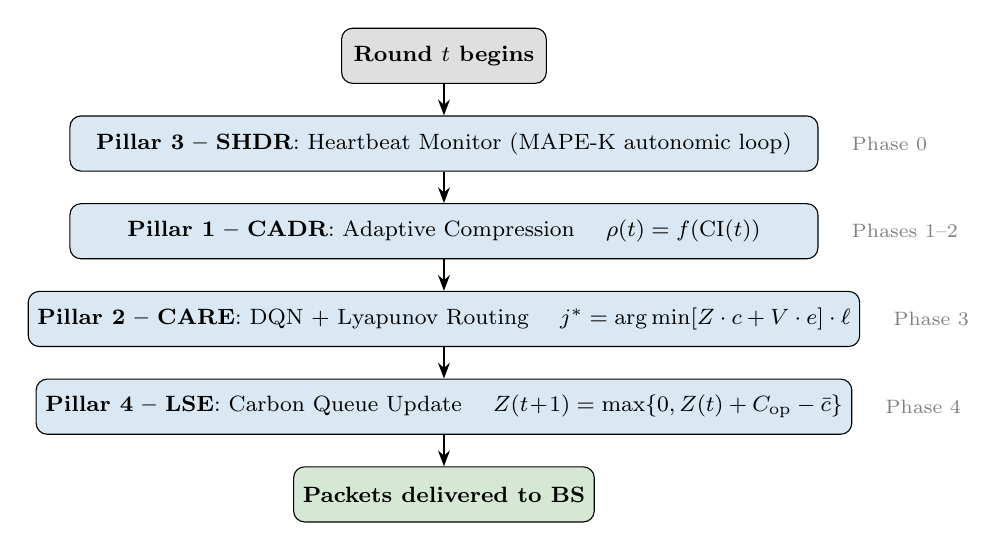
\begin{tikzpicture}[
    box/.style={draw, rounded corners, minimum width=2.6cm, minimum height=0.7cm, align=center, font=\footnotesize},
    pillar/.style={box, fill=calash!15, minimum width=9.5cm},
    arrow/.style={-{Stealth[length=2mm]}, thick},
    node distance=0.4cm
]
\node[box, fill=gray!25] (round) {\textbf{Round $t$ begins}};
\node[pillar, below=of round] (shdr) {\textbf{Pillar 3 -- SHDR}: Heartbeat Monitor (MAPE-K autonomic loop)};
\node[pillar, below=of shdr] (cadr) {\textbf{Pillar 1 -- CADR}: Adaptive Compression \quad $\rho(t) = f(\text{CI}(t))$};
\node[pillar, below=of cadr] (care) {\textbf{Pillar 2 -- CARE}: DQN + Lyapunov Routing \quad $j^* = \arg\min [Z \cdot c + V \cdot e] \cdot \ell$};
\node[pillar, below=of care] (lse) {\textbf{Pillar 4 -- LSE}: Carbon Queue Update \quad $Z(t\!+\!1) = \max\{0, Z(t) + C_{\text{op}} - \bar{c}\}$};
\node[box, fill=okgreen!20, below=of lse] (out) {\textbf{Packets delivered to BS}};

\draw[arrow] (round) -- (shdr);
\draw[arrow] (shdr) -- (cadr);
\draw[arrow] (cadr) -- (care);
\draw[arrow] (care) -- (lse);
\draw[arrow] (lse) -- (out);

\node[right=0.3cm of shdr, font=\scriptsize, text=gray] {Phase 0};
\node[right=0.3cm of cadr, font=\scriptsize, text=gray] {Phases 1--2};
\node[right=0.3cm of care, font=\scriptsize, text=gray] {Phase 3};
\node[right=0.3cm of lse, font=\scriptsize, text=gray] {Phase 4};
\end{tikzpicture}
\end{frame}

\begin{frame}{Architecture -- 6G Enabling Technologies (Substrate)}
\begin{columns}[T]
\column{0.5\textwidth}
\textbf{Sub-THz Communication}
\begin{itemize}
    \item 140 GHz D-band, 10 GHz bandwidth
    \item OFDM: 2,048 sub-carriers, $\eta = 0.93$
    \item Intra-cluster range: 30 m
\end{itemize}

\vspace{3mm}
\textbf{Reconfigurable Intelligent Surface (RIS)}
\begin{itemize}
    \item $N_{\text{RIS}} = 64$ elements
    \item Cascaded Tx$\to$RIS$\to$Rx channel
    \item Practical impairments modelled:\\CSI error, beam misalignment, coupling
\end{itemize}

\column{0.5\textwidth}
\textbf{ISAC -- Integrated Sensing \& Communication}
\begin{itemize}
    \item Same OFDM waveform for data + sensing
    \item Range-Doppler processing ($\Delta r = 1.5$ cm)
    \item CFAR detection ($P_{\text{fa}} = 10^{-4}$)
    \item KL-divergence anomaly scoring
    \item 15\% energy overhead but faster disaster detection
\end{itemize}

\vspace{3mm}
\textbf{Key role:}\\
RIS-DRL baseline shares this same 6G substrate $\Rightarrow$ \textcolor{calash}{\textbf{any gap = CALASH's algorithmic contribution}}
\end{columns}
\end{frame}

% %%%%%%%%%%%%%%%%%%%%%%%%%%%%%%%%%%%%%%%%%%%%%%%%%%%%%%%%%%%%
\section{Methodology}
% %%%%%%%%%%%%%%%%%%%%%%%%%%%%%%%%%%%%%%%%%%%%%%%%%%%%%%%%%%%%

\begin{frame}{Methodology -- Simulation Setup}
\begin{columns}[T]
\column{0.5\textwidth}
\textbf{Network Parameters}
\begin{itemize}
    \item 200 nodes, $200 \times 200$ m$^2$
    \item BS at (100, 250)
    \item $E_0 = 0.5$ J per node
    \item 5,000 rounds
    \item Disaster at round 2,000 ($r_d = 100$ m)
\end{itemize}

\vspace{2mm}
\textbf{Statistical Rigour}
\begin{itemize}
    \item \textbf{30 independent seeds} (42--71)
    \item Mean $\pm$ 95\% CI ($t$-distribution)
    \item Wilcoxon signed-rank test ($\alpha = 0.05$)
\end{itemize}

\column{0.5\textwidth}
\textbf{13 Protocol Variants}
\begin{itemize}
    \item \textbf{7 baselines}: LEACH, LEACH-1hop,\\EE-LEACH, ABC-ACO, EERP,\\Q-Routing, RIS-DRL
    \item \textbf{CALASH}: full framework
    \item \textbf{5 ablations}:\\
    -NoCO2, -NoSH, -NoCADR,\\-NoLCI, -NoTHz
\end{itemize}

\vspace{2mm}
\textbf{Real Data Sources}
\begin{itemize}
    \item Intel Lab traces (2.3M readings)
    \item UK Carbon Intensity API (8,760 h)
    \item USGS ShakeMap (disaster calibration)
\end{itemize}
\end{columns}
\end{frame}

\begin{frame}{Methodology -- Problem Formulation}
\begin{block}{Minimize Lifecycle Carbon Intensity}
\[
\min_{\boldsymbol{\pi}} \; \text{LCI}(\boldsymbol{\pi}) = \frac{\sum_{i=1}^{N} C_{\text{emb}}^{(i)} + \sum_{t=1}^{T} C_{\text{op}}(t) + \sum_{i:\text{dead}} C_{\text{eol}}^{(i)}}{\sum_{t=1}^{T} D(t)}
\]
\end{block}

\textbf{Subject to:}
\begin{align*}
    E_i(t) &\geq 0 \quad \forall i, t  &\text{(energy non-negativity)} \\
    \frac{1}{T}\sum_{t=1}^{T} C_{\text{tot}}(t) &\leq \bar{c} + B/V  &\text{(Lyapunov carbon bound)} \\
    \text{NMSE}(\rho) &\leq \delta \quad &\text{(data fidelity threshold)}
\end{align*}

\vspace{2mm}
\textbf{Theoretical guarantee:} CDL Pareto Bound (Theorem 1) -- provable near-optimal delivery \textit{and} lifecycle carbon budget compliance via Lyapunov drift-plus-penalty.
\end{frame}

\begin{frame}{Methodology -- CADR: Carbon-Aware Data Reduction (Pillar 1)}
\textbf{Core idea:} Compress more when grid is dirty, less when grid is clean.

\vspace{2mm}
\begin{block}{Reference-Point CADR Mapping}
\[
\rho(t) = \begin{cases}
    \rho_{\max} - (\rho_{\max} - \rho_{\text{mid}}) \cdot \dfrac{\text{CI}(t) - \text{CI}_{\min}}{\text{CI}_{\text{base}} - \text{CI}_{\min}} & \text{if } \text{CI}(t) \leq \text{CI}_{\text{base}} \\[8pt]
    \rho_{\text{mid}} - (\rho_{\text{mid}} - \rho_{\min}) \cdot \dfrac{\text{CI}(t) - \text{CI}_{\text{base}}}{\text{CI}_{\max} - \text{CI}_{\text{base}}} & \text{if } \text{CI}(t) > \text{CI}_{\text{base}}
\end{cases}
\]
\end{block}

\vspace{2mm}
\begin{itemize}
    \item $\rho_{\min} = 0.3$ (max compression), $\rho_{\max} = 0.8$ (min compression)
    \item Uses compressive sensing + OMP recovery
    \item Intel Lab data: $\sim$1-sparse in DCT $\Rightarrow$ perfect fidelity ($F = 1.000$) at $\rho = 0.55$
    \item \textbf{Ablation: removing CADR = +59\% LCI} (dominant pillar)
\end{itemize}
\end{frame}

\begin{frame}{Methodology -- CARE: Routing Engine (Pillars 2--4)}
\begin{columns}[T]
\column{0.48\textwidth}
\textbf{Lyapunov Router (provable)}
\begin{itemize}[nosep]
    \item Virtual carbon queue:\\ {\small $Z(t\!+\!1) = \max\{0, Z(t) + C_{\text{op}} - \bar{c}\}$}
    \item Next-hop selection:\\ {\small $j^* = \arg\min_{j} [Z \cdot c_{ij} + V \cdot e_{ij}] \cdot \ell_j$}
    \item \textbf{Provable} carbon budget via CDL bound
\end{itemize}

\vspace{1mm}
\textbf{Lifecycle Penalty (Pillar 4 -- LSE)}
{\small $\ell_j = 1 + w_{\text{eol}} \cdot (1 - E_j/E_0)^2$}\\
{\scriptsize Discourages routing through near-death nodes.}

\column{0.48\textwidth}
\textbf{DQN Router (adaptive)}
\begin{itemize}[nosep]
    \item 9D state $\to$ 64 $\to$ 32 $\to$ Q-value
    \item NumPy-only Double DQN
    \item Online learning, no pre-training
    \item Multi-objective reward
    \item \textbf{Fallback}: Lyapunov during recovery
\end{itemize}

\vspace{1mm}
\textbf{SHDR (Pillar 3)}
\begin{itemize}[nosep]
    \item MAPE-K autonomic loop
    \item Heartbeat monitoring + CH re-election
    \item 50-round recovery window
\end{itemize}
\end{columns}
\end{frame}

% %%%%%%%%%%%%%%%%%%%%%%%%%%%%%%%%%%%%%%%%%%%%%%%%%%%%%%%%%%%%
\section{Results \& Discussion}
% %%%%%%%%%%%%%%%%%%%%%%%%%%%%%%%%%%%%%%%%%%%%%%%%%%%%%%%%%%%%

\begin{frame}{Results -- Main Results (30 Seeds, 13 Protocols)}
\centering
\begin{adjustbox}{max width=\textwidth}
\footnotesize
\begin{tabular}{l r@{$\,\pm\,$}l r@{$\,\pm\,$}l r@{$\,\pm\,$}l r@{$\,\pm\,$}l}
\toprule
\textbf{Protocol} & \multicolumn{2}{c}{\textbf{Half-Death} $\uparrow$} & \multicolumn{2}{c}{\textbf{PDR} $\uparrow$} & \multicolumn{2}{c}{\textbf{LCI} $\downarrow$} & \multicolumn{2}{c}{\textbf{Eff. (pkt/J)} $\uparrow$} \\
\midrule
LEACH           & 931  & 6   & 0.857 & 0.003 & 13.42 & 0.08 & 1,536 & 10 \\
LEACH-1hop      & 806  & 13  & 0.865 & 0.001 & 16.09 & 0.16 & 1,282 & 13 \\
EE-LEACH        & 1,266 & 11 & 0.638 & 0.002 & 13.54 & 0.07 & 1,525 & 9 \\
ABC-ACO         & 880  & 5   & \textbf{0.892} & 0.002 & 13.72 & 0.08 & 1,503 & 9 \\
EERP            & 1,244 & 12 & 0.646 & 0.006 & 13.21 & 0.07 & 1,561 & 8 \\
Q-Routing       & 1,225 & 10 & 0.636 & 0.002 & 14.01 & 0.08 & 1,473 & 8 \\
\midrule
RIS-DRL         & \textbf{1,764} & 15 & 0.794 & 0.002 & \textbf{7.89} & 0.07 & \textbf{2,647} & 26 \\
\rowcolor{calash!10}
\textbf{CALASH} & 1,486 & 14 & 0.829 & 0.006 & 8.99 & 0.10 & 2,323 & 24 \\
\bottomrule
\end{tabular}
\end{adjustbox}

\vspace{4mm}
\begin{columns}[T]
\column{0.5\textwidth}
\textbf{CALASH vs. LEACH:}
\begin{itemize}
    \item \textcolor{okgreen}{\textbf{+60\%}} lifetime (1,486 vs. 931)
    \item \textcolor{okgreen}{\textbf{+82.9\%}} PDR
    \item \textcolor{okgreen}{\textbf{-33\%}} LCI (8.99 vs. 13.42)
\end{itemize}
\column{0.5\textwidth}
\textbf{All comparisons:}
\begin{itemize}
    \item $p < 10^{-5}$ (Wilcoxon signed-rank)
    \item All 30 seeds consistent
    \item CALASH beats all 6 traditional baselines
\end{itemize}
\end{columns}
\end{frame}

\begin{frame}{Results -- CALASH vs.\ RIS-DRL: The Controlled Trade-off}
\begin{columns}[T]
\column{0.5\textwidth}
\textbf{RIS-DRL wins on:}
\begin{itemize}
    \item Lifetime: 1,764 vs. 1,486 (+18.7\%)
    \item LCI: 7.89 vs. 8.99 (-12.2\%)
\end{itemize}

\vspace{2mm}
\textbf{But RIS-DRL lacks:}
\begin{itemize}
    \item[\xmark] Carbon-budget compliance
    \item[\xmark] Disaster self-healing
    \item[\xmark] CI-adaptive compression
    \item[\xmark] ISO 14040 lifecycle integration
\end{itemize}

\column{0.5\textwidth}
\textbf{CALASH wins on:}
\begin{itemize}
    \item PDR: 0.829 vs. 0.794 (+4.3\%)
    \item \textbf{4 unique capabilities} (Table I)
    \item Provable carbon guarantee (Thm. 1)
\end{itemize}

\vspace{2mm}
\textbf{Ablation proof:}\\
CALASH-NoCO2 (no carbon awareness)\\closes LCI gap to just \textbf{3.4\%}\\
$\Rightarrow$ gap = \textit{price of carbon awareness},\\ not architectural weakness.
\end{columns}

\vspace{4mm}
\centering
\textcolor{calash}{\textbf{CALASH trades $\sim$16\% lifetime for carbon awareness + disaster resilience + provable guarantees}}
\end{frame}

\begin{frame}{Results -- Ablation Study (Pillar Hierarchy)}
\centering
\begin{adjustbox}{max width=0.9\textwidth}
\begin{tabular}{lccl}
\toprule
\textbf{Ablation} & \textbf{$\Delta$ LCI} & \textbf{$\Delta$ Lifetime} & \textbf{Interpretation} \\
\midrule
\rowcolor{alertred!10}
CALASH-NoCADR & \textbf{+5.30} (+59\%) & $-37.4\%$ & \textbf{Dominant pillar} -- compression is key \\
CALASH-NoTHz  & +0.85 (+9.5\%) & $-9.5\%$ & 6G substrate = 2nd largest effect \\
CALASH-NoCO2  & $-0.83$ ($-9.2\%$) & $+10.7\%$ & Carbon awareness overhead (intended) \\
CALASH-NoSH   & $-0.17$ ($-1.9\%$) & $+1.7\%$ & Self-healing overhead (intended) \\
CALASH-NoLCI  & +0.00 (0\%) & $\approx 0\%$ & Gentle tiebreaker (by design) \\
\bottomrule
\end{tabular}
\end{adjustbox}

\vspace{3mm}
\textbf{Hierarchy:} CADR (+59\%) $\gg$ 6G (+9.5\%) $>$ CARE ($-9.2\%$) $>$ SHDR ($-1.9\%$) $>$ LSE ($\approx 0$)

\vspace{1mm}
\textcolor{calash}{\textbf{Key insight: sending fewer bits (CADR) is more effective than optimizing routing paths}}
\end{frame}

\begin{frame}{Results -- Key Figures}
\begin{columns}[T]
\column{0.5\textwidth}
\centering

\includegraphics[width=0.92\textwidth, height=0.33\textheight, keepaspectratio]{alive_nodes.pdf}\\
{\scriptsize Alive nodes -- CALASH recovers fastest after disaster}

\vspace{1mm}

\includegraphics[width=0.92\textwidth, height=0.33\textheight, keepaspectratio]{fig_ablation.pdf}\\
{\scriptsize Ablation: CADR is the dominant pillar}

\column{0.5\textwidth}
\centering

\includegraphics[width=0.92\textwidth, height=0.33\textheight, keepaspectratio]{pdr_curves.pdf}\\
{\scriptsize Cumulative PDR -- CALASH sustains high delivery}

\vspace{1mm}

\includegraphics[width=0.92\textwidth, height=0.33\textheight, keepaspectratio]{boxplots.pdf}\\
{\scriptsize Box plots: 30-seed consistency}
\end{columns}
\end{frame}

\begin{frame}{Results -- Supplementary Analyses}
\begin{columns}[T]
\column{0.5\textwidth}
\centering

\includegraphics[width=0.9\textwidth, height=0.33\textheight, keepaspectratio]{scalability.pdf}\\
{\scriptsize \textbf{Scalability}: 100--500 nodes, 17\%--40\% lower LCI}

\vspace{1mm}

\includegraphics[width=0.9\textwidth, height=0.33\textheight, keepaspectratio]{sensitivity.pdf}\\
{\scriptsize \textbf{Sensitivity}: robust ($\pm$15\% LCI max variation)}

\column{0.5\textwidth}
\centering

\includegraphics[width=0.9\textwidth, height=0.33\textheight, keepaspectratio]{fig_wilcoxon_heatmap.pdf}\\
{\scriptsize \textbf{Statistical significance}: all $p < 10^{-5}$}

\vspace{1mm}

\includegraphics[width=0.9\textwidth, height=0.33\textheight, keepaspectratio]{carbon_emissions.pdf}\\
{\scriptsize \textbf{Carbon grid}: France to India, 31\%--41\% advantage}
\end{columns}
\end{frame}

% %%%%%%%%%%%%%%%%%%%%%%%%%%%%%%%%%%%%%%%%%%%%%%%%%%%%%%%%%%%%
\section{Conclusion}
% %%%%%%%%%%%%%%%%%%%%%%%%%%%%%%%%%%%%%%%%%%%%%%%%%%%%%%%%%%%%

\begin{frame}{Conclusion -- Contributions}
\begin{enumerate}
    \item[\textbf{C1}] \textbf{CALASH framework}: first WSN protocol jointly minimizing lifecycle carbon intensity through 4 integrated pillars + 6G substrate

    \item[\textbf{C2}] \textbf{CADR}: novel carbon-modulated compressive sensing\\$\Rightarrow$ \textbf{dominant pillar} (+59\% LCI when removed)

    \item[\textbf{C3}] \textbf{CARE}: hybrid Lyapunov--DQN with \textbf{provable} CDL Pareto bound\\$\Rightarrow$ guaranteed carbon-budget compliance

    \item[\textbf{C4}] \textbf{Comprehensive evaluation}: 30 seeds $\times$ 13 protocols $\times$ 5,000 rounds\\$\Rightarrow$ \textbf{+60\%} lifetime, \textbf{-33\%} LCI, \textbf{82.9\%} PDR vs. LEACH ($p < 10^{-5}$)
\end{enumerate}

\vspace{4mm}
\begin{block}{Key Insight}
\centering
\textit{Sending fewer bits} (via compressive sensing) is more effective for reducing WSN carbon footprint than optimizing routing paths alone.
\end{block}

\vspace{2mm}
\centering
\textbf{Target journal:} IEEE Transactions on Green Communications and Networking
\end{frame}

\begin{frame}{Bilan -- Progress \& Roadmap}
\begin{columns}[T]
\column{0.48\textwidth}
\begin{block}{\textbf{Completed (Article 2)}}
\begin{itemize}[nosep]
    \item[\cmark] CALASH framework: 4 pillars + 6G
    \item[\cmark] Full Python codebase (19 modules)
    \item[\cmark] V5 campaign: 30 seeds $\times$ 13 protocols $\times$ 5,000 rounds
    \item[\cmark] 5 supplementary campaigns (scalability, sensitivity, carbon grid, etc.)
    \item[\cmark] 8 publication-quality figures
    \item[\cmark] 32-page article (IEEE TGCN format)
    \item[\cmark] Article ready for submission
\end{itemize}
\end{block}

\column{0.48\textwidth}
\begin{alertblock}{\textbf{Next Steps (Article 3 -- 1 week)}}
\begin{itemize}[nosep]
    \item Close the RIS-DRL gap: lightweight linear policy
    \item ISAC passive failure detection
    \item Hardware testbed: ESP32-S3 + LoRa
    \item Multi-disaster evaluation (3--5 events)
    \item Energy harvesting integration
    \item ns-3 co-simulation
\end{itemize}
\end{alertblock}

\vspace{2mm}
\centering
\textcolor{calash}{\textbf{Target: Article 3 draft by March 18, 2026}}
\end{columns}
\end{frame}

% %%%%%%%%%%%%%%%%%%%%%%%%%%%%%%%%%%%%%%%%%%%%%%%%%%%%%%%%%%%%
\section{Bibliography}
% %%%%%%%%%%%%%%%%%%%%%%%%%%%%%%%%%%%%%%%%%%%%%%%%%%%%%%%%%%%%

\begin{frame}[allowframebreaks]{Key References}
\footnotesize
\begin{thebibliography}{20}

\bibitem{heinzelman2000} W.~Heinzelman \textit{et al.}, ``Energy-efficient communication protocol for wireless microsensor networks,'' \textit{HICSS}, 2000.

\bibitem{bakaraniya2013} E.~Bakaraniya and S.~Mehta, ``K-LEACH: An improved LEACH protocol for lifetime improvement in WSN,'' \textit{IJST}, vol.~6, no.~5, 2013.

\bibitem{elkhediri2024} S.~El Khediri \textit{et al.}, ``Hybrid ABC-ACO for energy-efficient WSN routing,'' \textit{IEEE Access}, 2024.

\bibitem{biswas2018} S.~Biswas \textit{et al.}, ``Energy-efficient routing in WSNs,'' in \textit{Handbook of Research on WSN}, Springer, 2018.

\bibitem{boyan1994} J.~Boyan and M.~Littman, ``Packet routing in dynamically changing networks: A reinforcement learning approach,'' \textit{NeurIPS}, 1994.

\bibitem{akram2025} T.~Akram \textit{et al.}, ``EEMLCR: Machine-learning clustering with energy-efficient routing,'' 2025.

\bibitem{wang2025} J.~Wang \textit{et al.}, ``Fuzzy-DRL for distributed cluster-based routing,'' 2025.

\bibitem{freitag2021} C.~Freitag \textit{et al.}, ``The real climate and transformative impact of ICT,'' \textit{Patterns}, vol.~2, no.~3, 2021.

\bibitem{pirson2021} T.~Pirson and D.~Bol, ``Assessing the embodied carbon footprint of IoT edge devices,'' \textit{Green Computing}, 2021.

\bibitem{erdelj2017} M.~Erdelj \textit{et al.}, ``Wireless sensor networks and multi-UAV systems for natural disaster management,'' \textit{Computer Networks}, 2017.

\bibitem{neely2010} M.~J.~Neely, ``Stochastic network optimization with application to communication and queueing systems,'' \textit{Morgan \& Claypool}, 2010.

\bibitem{candes2006} E.~Cand\`{e}s \textit{et al.}, ``Robust uncertainty principles: exact signal reconstruction from highly incomplete information,'' \textit{IEEE TIT}, 2006.

\bibitem{huang2020} C.~Huang \textit{et al.}, ``Reconfigurable intelligent surfaces for energy efficiency in wireless communication,'' \textit{IEEE JSAC}, 2020.

\bibitem{mnih2015} V.~Mnih \textit{et al.}, ``Human-level control through deep reinforcement learning,'' \textit{Nature}, 2015.

\bibitem{iso14040} ISO~14040:2006, ``Environmental management -- Life cycle assessment -- Principles and framework.''

\end{thebibliography}
\end{frame}

% ============================================================
%  THANK YOU
% ============================================================
\begin{frame}[plain]
\centering
\vspace{2cm}
{\Huge\textcolor{calash}{\textbf{Thank You}}}

\vspace{1cm}
{\Large Questions?}

\vspace{1.5cm}
{\small Code \& data: \url{https://github.com/gedji2024/CALASH1}}
\end{frame}

\end{document}
